% This file was created by tikzplotlib v0.9.2.
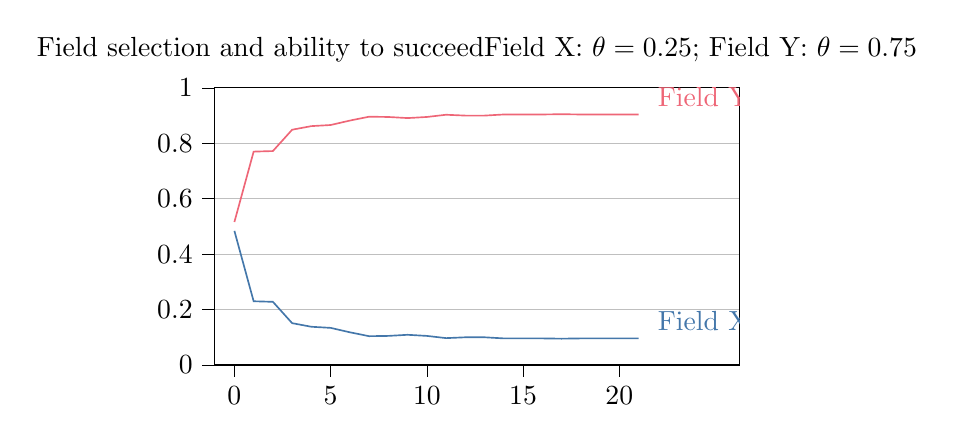
\begin{tikzpicture}

\definecolor{color0}{rgb}{0.266666666666667,0.466666666666667,0.666666666666667}
\definecolor{color1}{rgb}{0.933333333333333,0.4,0.466666666666667}

\begin{axis}[
height=5.101085673964669cm,
tick align=outside,
tick pos=left,
title={Field selection and ability to succeed \\ Field X: \(\displaystyle \theta=0.25\); Field Y: \(\displaystyle \theta=0.75\)},
width=8.25373cm,
x grid style={white!69.0196078431373!black},
xmin=-1.05, xmax=26.25,
xtick style={color=black},
xtick={0,5,10,15,20},
xticklabels={\(\displaystyle 0\),\(\displaystyle 5\),\(\displaystyle 10\),\(\displaystyle 15\),\(\displaystyle 20\)},
ymajorgrids,
ymin=0, ymax=1,
ytick style={color=black},
ytick={0,0.2,0.4,0.6,0.8,1},
yticklabels={\(\displaystyle 0\),\(\displaystyle 0.2\),\(\displaystyle 0.4\),\(\displaystyle 0.6\),\(\displaystyle 0.8\),\(\displaystyle 1\)}
]
\addplot [semithick, color0]
table {%
0 0.484
1 0.23
2 0.228
3 0.151
4 0.138
5 0.134
6 0.118
7 0.104
8 0.105
9 0.109
10 0.105
11 0.097
12 0.1
13 0.1
14 0.096
15 0.096
16 0.096
17 0.095
18 0.096
19 0.096
20 0.096
21 0.096
};
\addplot [semithick, color1]
table {%
0 0.516
1 0.77
2 0.772
3 0.849
4 0.862
5 0.866
6 0.882
7 0.896
8 0.895
9 0.891
10 0.895
11 0.903
12 0.9
13 0.9
14 0.904
15 0.904
16 0.904
17 0.905
18 0.904
19 0.904
20 0.904
21 0.904
};
\draw (axis cs:21.5,0.126) node[
  anchor=base west,
  text=color0,
  rotate=0.0
]{Field X};
\draw (axis cs:21.5,0.934) node[
  anchor=base west,
  text=color1,
  rotate=0.0
]{Field Y};
\end{axis}

\end{tikzpicture}
